Master's theses are, in many cases, just a small piece of effort
taking part in a more-widely scoped project. They generally lead to immature
research results which might need to be further-polished or, quite
oftenly, consist in continuing the work of yet another thesis. Thus,
they are generally subject to be extended and modified.

However, when it comes to practical results such us source code, they
tend to be weakly documented, hindering the first steps of a potential
future developer.

The main purpose of this guide is to help contributors getting
involved with the implementation details of the compiler and to save
them having to figure out the steps required to carry out the most
common extensions.
 
\section{Prerequisites}

In order to understand the compiler's code, a developer is obviously
required to be fluent in Haskell98 \cite{haskell}. It is also advisable
to have some experience with \texttt{mtl} (\textit{Monad Transformer
  Library}) which is extensively used throughout the sources.

Furthermore, in order to understand the full source code tree, it is assumed
that he (or she) will be familiar with common Haskell extensions such as
MPTC \cite{fundep} (\textit{Multi-parameter Type Classes}), Existential Types
and Template Haskell \cite{metahaskell}, which unfortunately, by the time of
writing this thesis are not still documented in a friendly way. The best
current resource to get familiar with them is the GHC User's
Guide \cite{ghc:guide}. However, the upcoming publication of a promising (and
free) book, \textit{Real-World Haskell} \cite{realworldhaskell}, covering those
extensions will certainly be helpful. Even though, there still could be
certain small tasks whose accomplishment should not necessarily rely on the
aforementioned extensions.

Being familiar with VHDL is specifically required to understand the
copmiler's VHDL backend. It is advisable to have access of the
VHDL93 \cite{vhdl93} standard, or other exhaustive reference material
before trying to extend this backend.



The compiler was developed and tested with GHC version 6.6 under a
GNU/Linux system\footnote{Although it was not tested under other
  operating systems, any development environment with GHC support
  could in theory be used.}.  The use of non-standard extensions make
it GHC-dependant and will eventually lead to regression problems which
will have to be addressed before performing extensions or even making
use of it.



Lastly, this guide is not self-contained, it complements the rest of
the thesis (especially chapter \ref{chap:design}) and was isolated in
an appendix due to covering specific implementation details not
considered of general-interest. Therefore, in order to understand this
guide, it will be assumed that the reader had already gone through the
rest of the thesis report.

\section{Compiler modules overview}

Figure \ref{fig:graph} contains the module dependency graph of the compiler.

\texttt{HD} is the main module, it stands for \textit{Hardware
  Description} and its purpose is simply to re-export other modules
(simplifying the importing task for the end-user) and to hide certain
implementation details to the outside world.

The rest of the modules will be explained in the next sections, where
they are grouped according to their functionality.

It is highly advisable to follow the same module-order when getting
familiar with the compiler in order to be able to understand it in an
incremental manner.

\subsection{Core modules}

They constitute the heart of the compiler and are the ones to be studied in
first place.

\begin{itemize}
\item \texttt{\textbf{HD.Types}}. This module contains the mechanisms
  and definitions related to the possible value-types which a signal
  (or more accurately an \texttt{HDSignal}) can
  carry\footnote{\texttt{Bool} and \texttt{Int} at the moment of
    writing this appendix.} and the type-representation of a function
  (\texttt{HDFunType}). 

  Basically, a signal can transport values of any type belonging to
  the class \texttt{HDPrimType}, standing for \textit{Hardware
    Description Primary Type}.


\begin{landscape}
\begin{figure}
\centering
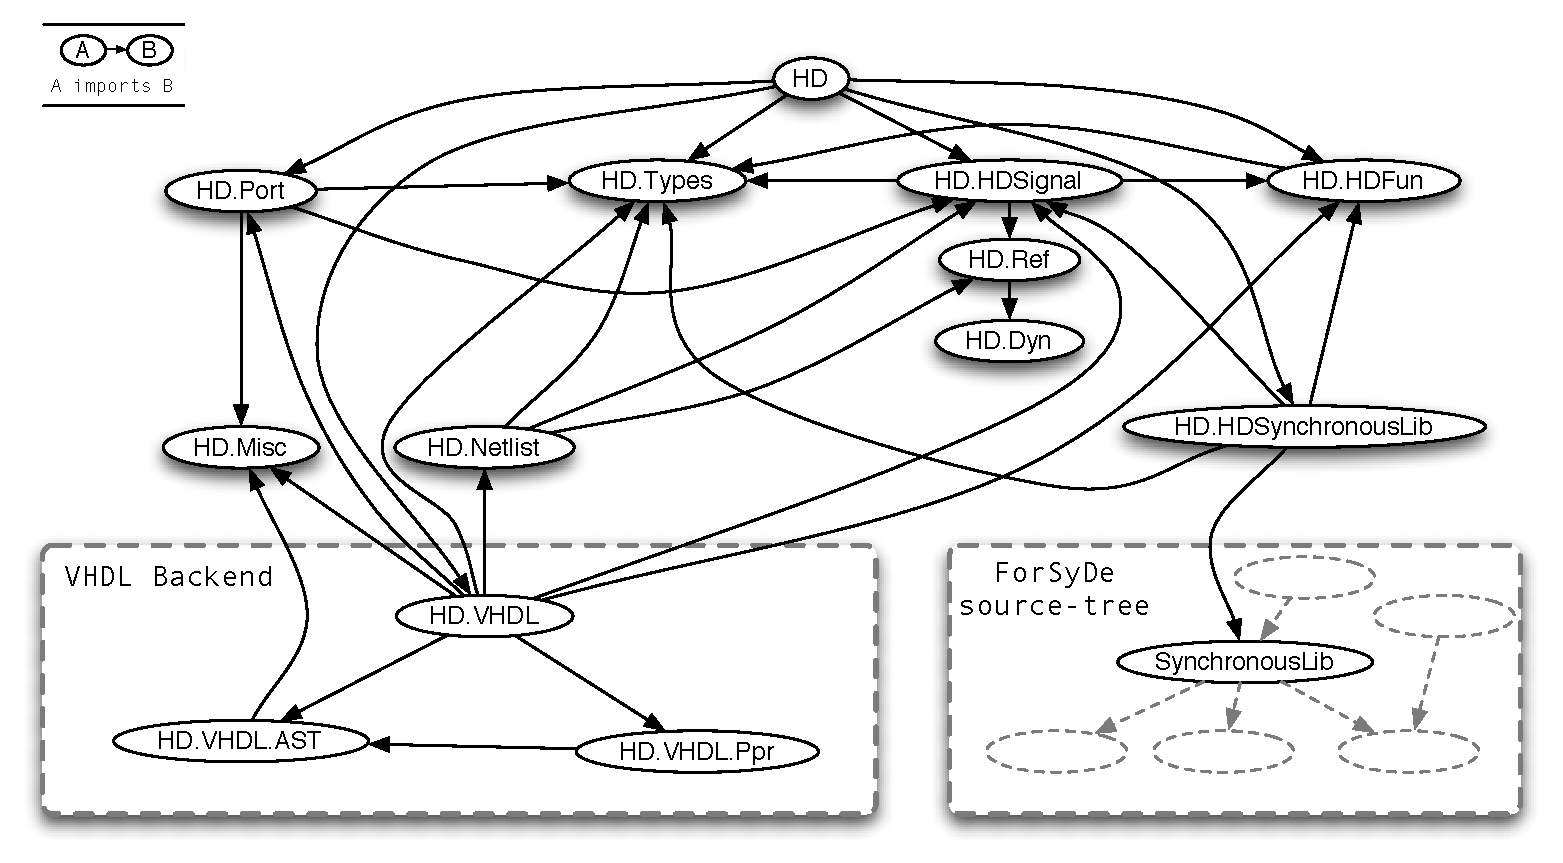
\includegraphics[height=.8\textwidth]{graph.pdf}
  \caption{Compiler modules' dependency graph}
  \label{fig:graph}
\end{figure}
\end{landscape}


\item \texttt{\textbf{HD.HDSignal}}. It is, without doubt, the most important
  module. It contains the definition of the user-hidden
  \textit{Hardware Description Signal}. 


  
  As it was previously mentioned, an \texttt{HDSignal}
  \textit{secretly} stores the structure of the circuit for latter
  processing, it is the compiler's intermediate representation of a
  circuit-description, and thus, it is the only usable information
  which a backend can work with.

  An \texttt{HDSignal} uses the same signal approach as
  Lava \cite{lava}, called \textit{Observable Sharing} \cite{osharing}
  which was earlier introduced in chapter \ref{chap:vs}.  Actually,
  both the modules \texttt{\textbf{HD.Ref}} (the Observable Sharing
  implementation) and \texttt{\textbf{HD.Dyn}} (unsafe dynamic types,
  used internally in \texttt{HD.Ref}) were taken and adapted from the
  Lava distribution.

  It is encouraged to fully understand the details of this module before
  attempting to extend the compiler or even trying to understand any other
  part of the source tree.

\item \texttt{\textbf{HD.HDFun}}. Most of the ForSyDe process
  constructors, such as $\mathit{mapSY}$ (see chapter
  \ref{chap:intro}) are represented in terms of a higher order
  function. That is, a function is passed along with the signal in
  order process it.
  
  The syntactical information of those functions needs to be
  internally stored (bundled with an \texttt{HDSignal}) for latter
  translation to the target language. The \texttt{HD.HDFun} module
  makes use of Template Haskell to make it possible: It provides a
  data structure (\texttt{HDFun}) which stores all the function
  information and a constructor (\texttt{mkHDFun}) to create such
  structure from the Template-Haskell representation
  (~\texttt{Q[Dec]}) of a function.  Colaterally, \texttt{HD.HDFun} is
  responsible of establishing the Haskell syntax-subset supported by
  \texttt{HDFun}s.

  Familiarity with Template Haskell is obviously a must in order to
  deal with this module.
\end{itemize}

\subsection{Miscellaneous auxiliary functions and types}

\texttt{\textbf{HD.Misc}} contains miscellaneous helper functions and
types which are too small to be splitted in their own modules.  The
only important part to highlight is the \texttt{EProne a} type, which
holds an \textit{error-prone} value and uses \texttt{mtl}'s
\texttt{Error} monad class to handle those errors.
  
Error management within the compiler is handled, to a large extend,
through the \texttt{Eprone} type.

\subsection{Ports, Blocks and Block Instances}
The concepts of a \textit{Port},\textit{Block} and \textit{Block
  Instance} were introduced in chapter \ref{chap:design}. The
\texttt{HD.Port} module implements them and enables their use,
providing as well an API to the end-user to deal with them.

The introduction of Ports has implied as well the introduction of
typecheking (there is no way to statically assure whether a the type
of a port entry matches a signal attached to it).

Moreover, due to the fact that the compiler is Embedded in Haskell,
compilation of the guest language (i.e. ForSyDe models) strangely
takes place at runtime, and unavoidably so does typechecking. 

As a result, the functions which attach or obtain signals to/from a
port (namely \texttt{plugSig} and \texttt{supplySig}) are in charge of doing
typechecking.

Moreover, due to the restrictions imposed by the host language,
typechecking turns to be a difficult task. A tricky solution using
dynamic signals (that is, \texttt{forall}\footnote{If you are confused
  with the \texttt{forall} keyword, that means you should 
  get familiar with existential types before trying to go through this
  module.}\texttt{a.HDPrimType a => HDSignal a}) was figured out. It
works nicely in practice, but it certainly could (and probably should)
be redesigned or improved.

The coexistence of static and dynamic signals requires a way of
conversion between them. That is the purpose of the \texttt{sigCast} function.

\subsection{Backends}
\label{backends}
A backend is in charge of interpreting the intermediate representation
of the source code. The most common form of interpretation is a
translation into another language (e.g.  \texttt{VHDL}) but some other
possibilities are: simulation, design verification, generation of a graphical
representation etc $\dots$. 

In our case, a backend uses a \texttt{Block} as input, whose netlist
(the internal circuit graph) is traversed to achieve the
aforementioned interpretation. 

The module \texttt{HD.NetList} (which was imported and adapted from
Lava) provides the developer with \texttt{netlist}, a function which
carries out the traversal of the circuit. Due to the use of
\textit{Observable Sharing} in the circuit representation, which is
right now is restricted to \texttt{IO}-references (see module
\texttt{HD.Ref}) \texttt{netlist} is subdued to the \texttt{IO} Monad.
Furthermore, in order to allow reading and modifying state data during
the traversal, the \texttt{IO} Monad is wrapped into \texttt{mtl}'s
\texttt{StateT} monad transformer.

There could be interpretations, such as simulation, for which a
\texttt{ST} version of \texttt{netlist} would be preferable to current
\texttt{IO} version. Adding an alternative \texttt{ST} version would
involve including \texttt{ST}-references in \texttt{HD.Ref} (maybe
from the Lava-project, which already offers them).

Currently, the only available backend is a translator to VHDL, which
is divided in three modules

\begin{itemize}
\item \texttt{\textbf{HD.VHDL}}. It is in charge of the VHDL translation,
  which is accessible through the \texttt{writeVHDL} function.

\item \texttt{\textbf{HD.VHDL.AST}} defines data structures to hold
  the AST (\textit{Abstract Syntax Tree}) of the generated VHDL modules.  

  It is based in the grammar of the VHDL93 standard but only supports
  the subset of VHDL's syntax which has been needed. However, due to
  being based in the standard it could be easily extended in the
  future if desired.
  
\item \texttt{\textbf{HD.VHDL.Ppr}}. A \texttt{pretty-printer} library
  for the VHDL AST-structures mentioned above. It is in charge of the
  transformation and output of the AST into readable VHDL text
  modules.

\end{itemize}

\subsection{Integration with ForSyDe}

The development of the compiler did not entail big changes in
the ForSyDe library. A new alternative signal type (\texttt{HDSignal})
was developed to avoid modifying ForSyDe's original stream-based
\texttt{Signal} type.

However, one of the main compiler design-requirements was to be able
to reuse the original name and semantics of ForSyDe's
signal-processing functions with the new signal type.  It is a
certainly nice feature, since it allows all earlier documentation to
still apply for both signal types. In order to make it possible,
ForSyDe's original \texttt{SynchronousLib} module had to be modified.
Its \texttt{mapSY}, \texttt{zipWithSY} and \texttt{delaySY} functions
(the only ForSyDe processes currently supported natively by the
compiler) were transformed into type classes\footnote{Due to the
  nature of the the signal processing functions, the type classes
  required various parameters, and thus \textit{Multiparameter Type
    Classes} (a common Haskell extension) where used for that
  purpose.} and instances were created for both \texttt{Signal} and
\texttt{HDSignal}.

The new type classes and \texttt{Signal} instances remain in
\texttt{SynchronousLib} while the \texttt{HDSignal} ones were included
in a new module: \texttt{HDSynchronousLib}.

It is worth to note that, even if the compiler only currently supports
$\mathit{mapSY}$, $\mathit{zipWithSY}$ and $\mathit{delaySY}$ natively
as primitives\footnote{It can be said that they constitute the
  primitive processes of the compiler.}, due to the type class scheme
described above, all their derived process constructors (e.g.
$\mathit{sourceSY}$), are automatically supported.  However they are
treated as compound processes and thus, there is currently no way to
internally identify them as individual entities.  Treating those
derived processes as primitives would be desirable for a more precise
control of the way in which the design is interpreted, allowing
optimizations and improving code generation in the backends.

\section{Recipes to extend the compiler}

The following sections are targeted at suggesting the steps to follow
when developing common extensions for the compiler. 

The main purpose of these recipes is to help new developers, only
interested in certain extensions, to get familiar with the compiler.
Depending on the extension, some other changes might be required. As a
result, it is encouraged to take the recipes with a grain of salt and
expect further modifications to be needed in the process.

\subsection{Adding support for new types of signal values}

\texttt{Bool} and \texttt{Int} \texttt{HDSignal}s might be enough for
many designs, but it can be a good idea to support other signal values such as
tuples, enumerates etc $\dots$

To add a new type, say \texttt{a}

\begin{enumerate}[1)]
\item Add a constructor for \texttt{a} in \texttt{HD.HDTypes.HDType}
\item Make \texttt{a} an instance of \texttt{HD.HDTypes.HDPrimType}
\item Add a constructor for \texttt{a} in \texttt{HD.HDTypes.HDPrimConst}
\item Adjust the backends to handle the new type. In the VHDL backend
  that roughly means changing \texttt{HD.VHDL.hDST2TM} and
  \texttt{HD.VHDL.hDPC2Expr}.
\item The new type might require extending the Haskell subset
  supported by \texttt{HDFun}s. For instance, tuples would be difficult to
  use without pattern matching. Read on for details about how to perform
  this extension.
\item Consider adding support for new functions within an
  \texttt{HDFun}.  As an example, in the case of choosing to add
  support for tuples, it would be desirable to get support for
  well-known \texttt{fst} and \texttt{snd} functions.  Details about
  how to do this are covered in a following section.
\end{enumerate}

\subsection{Treating more ForSyDe processes as primitives}

As it was previously stated, the only process constructors treated
natively as primitives are $\mathit{mapSY}$, $\mathit{zipWithSY}$ and
$\mathit{delaySY}$.  $\mathit{sourceSY}$, for example, is handled as a
compound of $\mathit{mapSY}$ and $\mathit{delaySY}$.

In order to treat a process, say $\mathit{sourceSY}$ from ForSyDe's
original \texttt{SynchronousLib}, as a primitive:

\begin{enumerate}[1)]
\item Add \texttt{sourceSY} to \texttt{HD.HDSignal.HDSignal}
\item Transform \texttt{SynchronousLib.sourceSY} into a type class and use
  its previous definition to make \texttt{Signal} an instance of it.
\item Modify \texttt{HD.HDSynchronousLib} by making \texttt{HDSignal}
  an instance of the new \texttt{SourceSY} class.
\item Adjust the backends to handle the new primitive. Basically, that entails
  changing the \texttt{new} and \texttt{define} functions passed to
  \texttt{netlist}, see \texttt{HD.VHDL} for more details.
\end{enumerate}

\subsection{Extending \texttt{HDFun}'s Haskell-syntax subset}
The Haskell syntax admited by \texttt{HDFun}s (more precisely by
\texttt{HD.HDFun.mkHDFun}) is quite limited. For example, neither
constructor pattern-matching nor \textit{where-clauses} are allowed
(chapter \ref{chap:design} gives a precise description of the supported
subset).

To broaden the supported Haskell-subset.

\begin{enumerate}[1)]
\item Locate what type in the the Template Haskell AST
  (\texttt{Language.Haskell.TH.Syntax}) holds the desirable syntax
  extension.
\item Modify the corresponding \texttt{Lift} instantiate for that type in
  \texttt{HD.HDFun}  in order to give support to the new feature.
\item Adapt the compiler backends to the change.
\end{enumerate}
 
\subsection{Adding support for new functions within \texttt{HDFun}s}
The functions which a designer can use within a \texttt{HDFun} (e.g.
\texttt{(\&\&)}, \texttt{(==)}, \texttt{(-)}, \texttt{(+)} $\dots$ )
are limited.  That limitation, however, is not intrinsic to
\texttt{HDFun}s themselves, which can indeed make use of any valid
Haskell function as long as it is done in a correct manner. The
problem is that those functions have to be interpreted at some point
by the translation backends.

Thus, in order to support new functions within an \texttt{HDFun}, the
backend has to be aware of them and know how to handle them.
For that reason, to add in a new function simply ...

\begin{itemize}
\item Adapt the backends to support the new function.
\end{itemize}

The way to dispatch those functions depends highly on the translation
backend, for example, in the \texttt{VHDL} backend, translation tables
are kept to help mapping them from Haskell to VHDL.

A simulation backend on the other hand does not involve a translation
and could make use of the original Haskell function (which is stored
in the \texttt{HDFun} algebraic type). That makes possible to forget
about the \texttt{HDFun} AST and translation tables.

\subsection{Adding a new backend}

To add a new backend such as simulation, translation to another target
language or code verification, the intermediate representation the ForSyDe
model has to be traversed and processed. A good way to start up would be
looking at the sources of current \texttt{VHDL} backend to understand how the
\texttt{netlist} function works in practice.

A simulation backend could be coded as follows.

\begin{enumerate}[1)]
\item Verify whether the \texttt{HD.NetList.netlist} function fulfils
  the needs of the backend and otherwise create an alternative version.

  Simulation could serve as a means of translating between
  \texttt{HDSignal}s and \texttt{Signal}s but unfortunately
  \texttt{netlist} depends on \texttt{IO} from which no one can safely
  escape (transforming an \texttt{IO a} value into \texttt{a} 
  causes side effects). Thus, a
  \texttt{ST}-\texttt{netlist}\footnote{The \texttt{a} value of
    \texttt{ST a} can be extracted through \texttt{runST}} version
  would be necessary to bypass \texttt{IO}.  See section
  \ref{backends} for more details.

\item Check if the intermediate representation of the circuit
  (contained in \texttt{\texttt{HD.\-HDSignal.\-HDSignal}}) needs to
  be extended.
  
  A simulation backend would need to make use of the original Haskell
  function stored in \texttt{HDFun}s to avoid having to traverse its
  AST. However, the function itself is not stored in an \texttt{HDSignal}

\item Lastly, code the backend.
\end{enumerate}

\section{Improving the source code}

Every piece of software is an evolving entity which can always be
improved. The compiler produced during this thesis is no exception and
is far for being perfect in many ways.

Due to the time-limitation of the thesis, I was not able to make the
code be organized and work as good I would have liked to, but at least
I was careful enough to anotate and coment all the potential
improvements I could notice.  I used the traditional \texttt{FIXME}
and \texttt{TODO} tags for that purpose.

Reading the output produced by \texttt{grep -ri 'TODO$\backslash$|FIXME' *} in
the \texttt{HD} directory gives a good hint about where to start
working.

